\section{Results}

This section reports the frozen four-scenario benchmark and the same-noise
Transformer diagnostic. Validation checks confirmed the expected test seeds
\(1000\)--\(1049\) and reproduced the stored scenario summaries from per-series
outputs under the primary 25-step matching margin. Table~\ref{tab:main-benchmark-top5}
reports the top five methods per scenario; full leaderboards are kept in the
reproducibility package.

\begin{table}[t]
  \centering
  \caption{Top five methods by mean F1 in each frozen benchmark scenario.
  Precision (P), recall (R), F1, mean absolute localization error (MAE),
  ROC-AUC (ROC), and PR-AUC (PR) are reported when available.}
  \label{tab:main-benchmark-top5}
  \begin{tabular}{llllllll}
\toprule
Scenario & Method & P & R & F1 & MAE & ROC & PR \\
\midrule
D=0.5, white & SNHT & 1.000 & 0.641 & 0.725 & 1.360 &  &  \\
D=0.5, white & Chow & 0.920 & 0.561 & 0.645 & 4.520 & 0.684 & 0.533 \\
D=0.5, white & GRU\_v2 & 0.322 & 0.230 & 0.253 & 3.180 & 0.918 & 0.551 \\
D=0.5, white & CatBoost & 0.355 & 0.213 & 0.243 & 4.280 & 0.650 & 0.211 \\
D=0.5, white & LSTM\_v2 & 0.237 & 0.209 & 0.207 & 2.320 & 0.866 & 0.424 \\
D=1, white & Transformer\_v2 & 0.774 & 0.641 & 0.698 & 3.560 & 0.815 & 0.799 \\
D=1, white & LSTM\_v2 & 0.840 & 0.569 & 0.675 & 3.350 & 0.813 & 0.811 \\
D=1, white & GRU\_v2 & 0.913 & 0.511 & 0.650 & 3.690 & 0.847 & 0.850 \\
D=1, white & CUSUM & 0.462 & 0.645 & 0.534 & 9.790 & 0.483 & 0.467 \\
D=1, white & CatBoost & 0.921 & 0.325 & 0.479 & 2.290 & 0.733 & 0.788 \\
D=1, pink & Transformer\_v2 & 0.916 & 0.410 & 0.566 & 3.330 & 0.896 & 0.972 \\
D=1, pink & GRU\_v2 & 0.987 & 0.384 & 0.551 & 2.610 & 0.922 & 0.981 \\
D=1, pink & LSTM\_v2 & 0.981 & 0.354 & 0.520 & 2.100 & 0.870 & 0.966 \\
D=1, pink & CUSUM & 0.794 & 0.270 & 0.402 & 7.500 & 0.474 & 0.783 \\
D=1, pink & CatBoost & 0.850 & 0.124 & 0.216 & 1.610 & 0.666 & 0.915 \\
D=1.5, white & Transformer\_v2 & 0.964 & 0.483 & 0.643 & 3.210 & 0.810 & 0.960 \\
D=1.5, white & LSTM\_v2 & 0.956 & 0.438 & 0.599 & 3.590 & 0.807 & 0.960 \\
D=1.5, white & CUSUM & 0.845 & 0.461 & 0.595 & 7.980 & 0.458 & 0.837 \\
D=1.5, white & GRU\_v2 & 0.969 & 0.278 & 0.429 & 3.280 & 0.806 & 0.959 \\
D=1.5, white & CatBoost & 0.991 & 0.206 & 0.341 & 2.100 & 0.828 & 0.968 \\
\bottomrule
\end{tabular}

\end{table}

\begin{table}[t]
  \centering
  \caption{Bootstrap confidence intervals for mean F1, computed by resampling
  independent test series.}
  \label{tab:bootstrap-f1-ci}
  \begin{tabular}{lll}
\toprule
Scenario & Method & Mean F1 [95\% CI] \\
\midrule
D=0.5, white & SNHT & 0.725 [0.650, 0.800] \\
D=0.5, white & Chow & 0.645 [0.555, 0.733] \\
D=0.5, white & GRU\_v2 & 0.253 [0.182, 0.329] \\
D=0.5, white & CatBoost & 0.243 [0.175, 0.313] \\
D=0.5, white & LSTM\_v2 & 0.207 [0.144, 0.273] \\
D=1, white & Transformer\_v2 & 0.698 [0.682, 0.714] \\
D=1, white & LSTM\_v2 & 0.675 [0.652, 0.696] \\
D=1, white & GRU\_v2 & 0.651 [0.630, 0.670] \\
D=1, white & CUSUM & 0.534 [0.518, 0.551] \\
D=1, white & CatBoost & 0.479 [0.469, 0.490] \\
D=1, pink & Transformer\_v2 & 0.566 [0.555, 0.577] \\
D=1, pink & GRU\_v2 & 0.551 [0.541, 0.561] \\
D=1, pink & LSTM\_v2 & 0.520 [0.508, 0.530] \\
D=1, pink & CUSUM & 0.402 [0.391, 0.413] \\
D=1, pink & CatBoost & 0.216 [0.209, 0.222] \\
D=1.5, white & Transformer\_v2 & 0.643 [0.631, 0.655] \\
D=1.5, white & LSTM\_v2 & 0.599 [0.586, 0.612] \\
D=1.5, white & CUSUM & 0.595 [0.586, 0.603] \\
D=1.5, white & GRU\_v2 & 0.429 [0.412, 0.446] \\
D=1.5, white & CatBoost & 0.341 [0.334, 0.348] \\
\bottomrule
\end{tabular}

\end{table}

\begin{figure}[htbp]
  \centering
  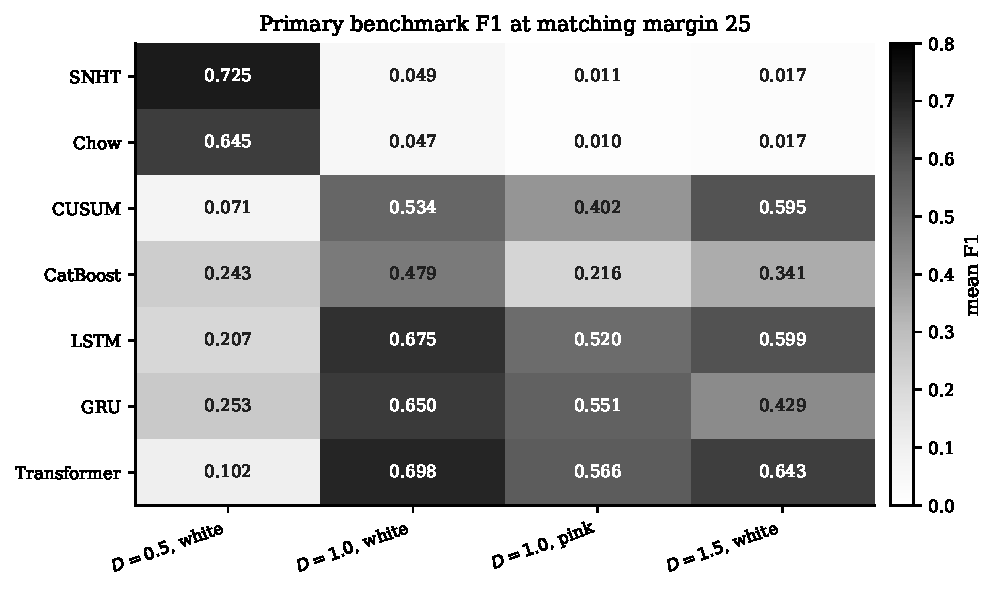
\includegraphics[width=\linewidth]{../assets/figures/fig02_primary_f1_benchmark.pdf}
  \caption{Primary benchmark F1 at the matching margin of 25 timesteps for the
  manuscript methods and frozen test scenarios. Classical tests lead in the
  sparse low-\(D\) setting; learned window-based detectors rank higher in the
  \(D=1.0\) and strict \(D=1.5\) evaluations.}
  \label{fig:primary-f1-benchmark}
\end{figure}

Table~\ref{tab:main-benchmark-top5} and Fig.~\ref{fig:primary-f1-benchmark}
separate the sparse low-\(D\) case from the larger-\(D\) cases. For \(D=0.5\)
with white noise, SNHT leads with mean F1 \(0.725\), followed by Chow at
\(0.645\); the strongest listed learned detector is far below this range. SNHT
also has low matched-event localization error, with MAE \(1.360\) timesteps.
For \(D=1.0\), learned window-based detectors rank higher: Transformer leads in
the white-noise and pink-noise scenarios, although the white-noise
Transformer--LSTM gap is qualified by the paired test below. For \(D=1.5\) with
white noise, Transformer leads under the primary 25-step margin, while LSTM and
CUSUM are close. The matching-margin robustness check shows that this ranking
is tolerance-sensitive: CUSUM overtakes Transformer when the evaluation
tolerance is widened to 50 or 100 timesteps.

\begin{figure}[htbp]
  \centering
  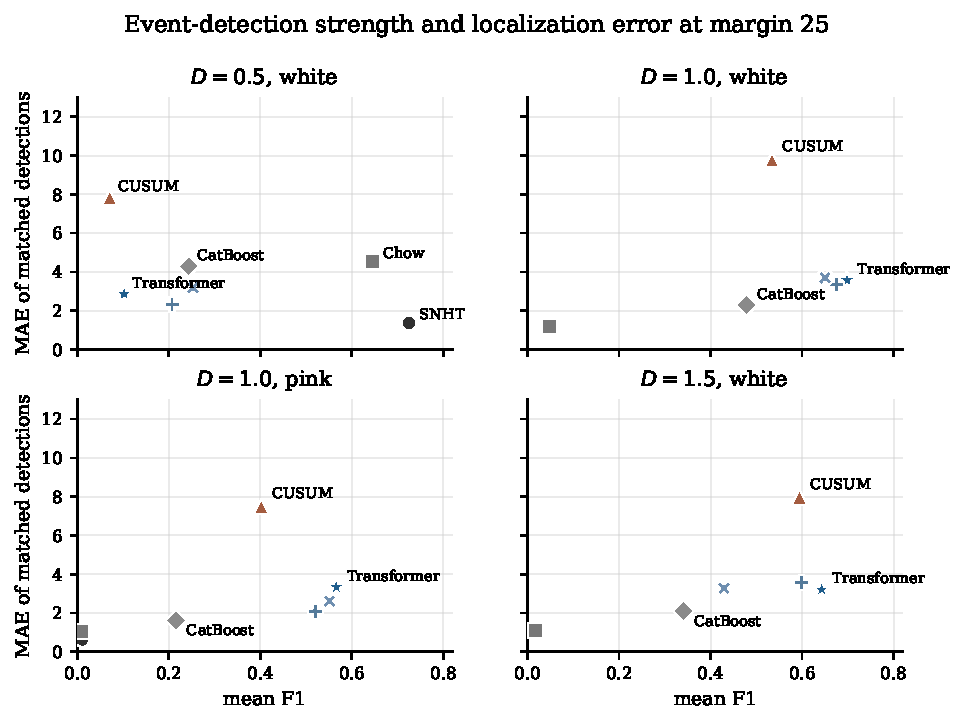
\includegraphics[width=\linewidth]{../assets/figures/fig04_f1_mae_tradeoff.pdf}
  \caption{Mean F1 and mean absolute localization error for selected methods at
  the primary matching margin. MAE is computed only for matched detections and
  should be read together with F1.}
  \label{fig:f1-mae-tradeoff}
\end{figure}

\begin{table}[t]
  \centering
  \caption{Paired Wilcoxon comparisons on per-series F1 for key method pairs.}
  \label{tab:paired-wilcoxon}
  \begin{tabular}{llllll}
\toprule
Scenario & A & B & Alt. & Mean F1 diff & p \\
\midrule
D=0.5, white & SNHT & Chow & greater & 0.080 & 0.0228 \\
D=0.5, white & SNHT & GRU\_v2 & greater & 0.472 & <0.0001 \\
D=1, white & Transformer\_v2 & CUSUM & greater & 0.164 & <0.0001 \\
D=1, white & Transformer\_v2 & GRU\_v2 & greater & 0.048 & <0.0001 \\
D=1, white & Transformer\_v2 & LSTM\_v2 & two-sided & 0.023 & 0.0937 \\
D=1, pink & Transformer\_v2 & CUSUM & greater & 0.164 & <0.0001 \\
D=1, pink & Transformer\_v2 & GRU\_v2 & two-sided & 0.015 & 0.0011 \\
D=1.5, white & Transformer\_v2 & CUSUM & greater & 0.048 & <0.0001 \\
D=1.5, white & Transformer\_v2 & LSTM\_v2 & two-sided & 0.044 & <0.0001 \\
\bottomrule
\end{tabular}

\end{table}

The paired tests in Table~\ref{tab:paired-wilcoxon} support the bounded ranking
claims. SNHT exceeds Chow and GRU in the \(D=0.5\), white-noise scenario. At
\(D=1.0\) with white noise, Transformer exceeds CUSUM and GRU, but the
Transformer--LSTM comparison remains close (\(p=0.0937\)). Under the primary
margin, Transformer exceeds CUSUM for \(D=1.0\) pink noise and \(D=1.5\) white
noise; the robustness pass qualifies the latter result because CUSUM improves
under wider tolerances.

\begin{figure}[htbp]
  \centering
  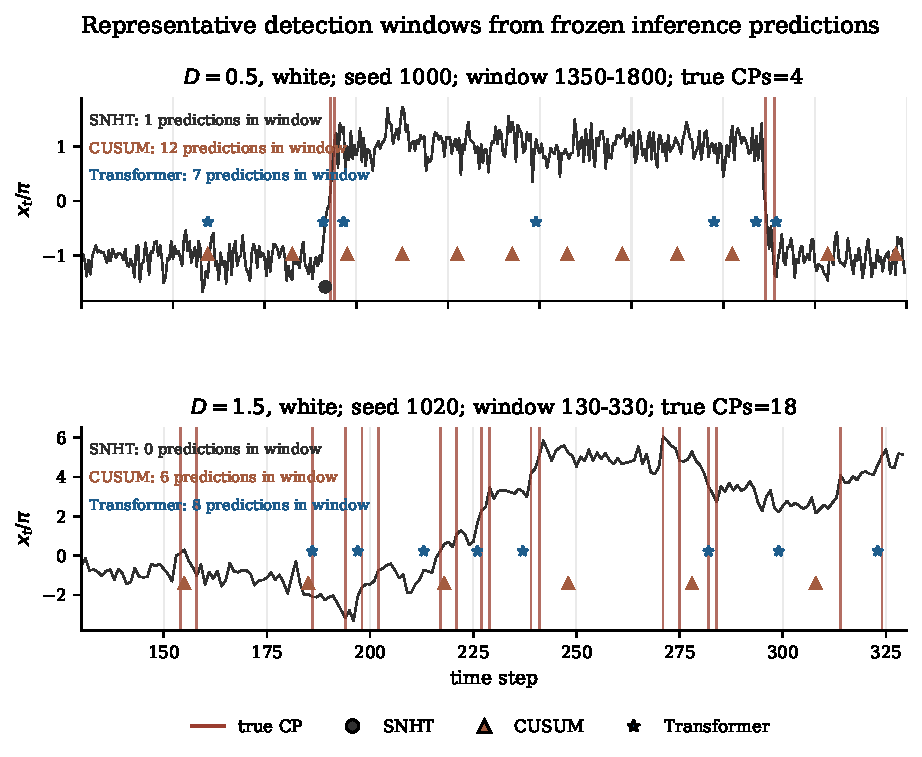
\includegraphics[width=\linewidth]{../assets/figures/fig05_detection_overlay.pdf}
  \caption{Representative detection windows. Vertical lines show true change
  points; markers show selected method predictions.}
  \label{fig:detection-overlay}
\end{figure}

\begin{table}[t]
  \centering
  \caption{Same-noise \(D=1.0\) diagnostic comparison against the best
  classical baseline on the same 50 test seeds.}
  \label{tab:same-noise-diagnostic}
  \begin{tabular}{llll}
\toprule
Noise & Transformer F1 & Classical F1 & Best classical method \\
\midrule
white & 0.586 & 0.663 & CUSUM \\
pink & 0.263 & 0.464 & CUSUM \\
brownian & 0.121 & 0.259 & CUSUM \\
blue & 0.160 & 0.523 & SNHT/Chow \\
violet & 0.078 & 0.793 & SNHT/Chow \\
\bottomrule
\end{tabular}

\end{table}

The same-noise experiment in Table~\ref{tab:same-noise-diagnostic} gives the
colored-noise boundary. Training and testing Transformer separately within each
\(D=1.0\) noise family still leaves it below the best classical baseline in all
five cases. Noise-specific Transformer training alone therefore does not support
a universal colored-noise neural-advantage claim under the evaluated pipeline.

